\documentclass[11pt,a4paper]{article}
\usepackage{microtype}
\usepackage{booktabs}
\usepackage{hyperref}
\usepackage{graphicx}
\usepackage{amsmath}
\usepackage{cleveref}
\usepackage[spanish]{babel}
\raggedbottom

\title{Reporte Técnico: Gatekeeping de Datos Shift-Left para Conjuntos de Datos de Visión por Computadora}
\author{William Steve Rodriguez Villamizar (wisrovi rodriguez)\\Líder de IA y Arquitecto de Soluciones\\wisrovi-suit (https://github.com/wisrovi/w-cli)}
\date{}

\begin{document}
\maketitle

\section{Resumen \& Palabras Clave}
\textbf{Resumen:} Enviar cargas de trabajo intensivas de visión por computadora a GPUs distribuidas incurre en costos económicos y temporales masivos cuando los procesos fallan a la mitad debido a conjuntos de datos corruptos. En entornos de almacenamiento en red compartido (CIFS/Samba), ontologías YAML malformadas o etiquetas YOLO faltantes provocan con frecuencia bloqueos en tiempo de ejecución horas después de iniciada una época de entrenamiento. Introducimos \texttt{wyoloservice2\_data\_prep}, un "Gatekeeper" automatizado adherido a la filosofía de IA Centrada en Datos. Al implementar una estrategia de validación Shift-Left, este servicio utiliza contenedores temporales para analizar y validar estáticamente conjuntos de datos en montajes remotos antes de la asignación de la GPU. Cuando se detecta corrupción, el trabajo se rechaza preventivamente y alertas automáticas de Slack notifican a los investigadores. Nuestro estudio empírico de ablación demuestra que la implementación de este gatekeeper Shift-Left redujo los ciclos de GPU desperdiciados en un 94\% y disminuyó el tiempo de depuración manual en 2.4 horas por incidente. Validar remotamente las estructuras de datos antes del entrenamiento es crítico para mantener la salud operativa de un clúster de ML multi-inquilino.

\textbf{Palabras Clave:} IA Centrada en Datos, Validación Shift-Left, MLOps, Clústeres de GPU Distribuidos, Calidad de Datos, wyoloservice.

\section{Información del Autor}
Esta investigación fue conceptualizada y desarrollada por William Steve Rodriguez Villamizar (wisrovi rodriguez), Líder de IA y Arquitecto de Soluciones para el ecosistema wisrovi-suit (https://github.com/wisrovi/w-cli).

\section{Introducción}
En los canales modernos de MLOps, los científicos de datos envían rutinariamente trabajos de entrenamiento a gran escala que referencian conjuntos de datos almacenados en unidades de red centralizadas (CIFS/Samba). Un cuello de botella persistente en la industria ocurre cuando estos conjuntos de datos contienen anomalías estructurales—tales como archivos \texttt{.txt} de bounding box faltantes, configuraciones YAML malformadas, o encabezados de imagen corruptos.

Los sistemas de orquestación estándar asignan una GPU, cargan el modelo en VRAM, y comienzan el entrenamiento. Si el punto de datos corrupto se encuentra en el percentil 80 del conjunto de datos, el ciclo de entrenamiento se ejecutará durante horas antes de fallar. Esta falla en etapa tardía desperdicia energía significativa, monopoliza recursos escasos de GPU, y requiere intervención humana para descifrar trazas de pila abstractas de PyTorch.

Abordamos esta ineficiencia desplazando la validación del conjunto de datos al comienzo mismo del ciclo de orquestación (Shift-Left). Desarrollamos un servicio de gatekeeper dedicado (\texttt{wyoloservice2\_data\_prep}) que monta dinámicamente el volumen remoto y ejecuta un análisis estructural estático del conjunto de datos. Si el conjunto de datos falla esta rigurosa verificación de salud, el trabajo es rechazado antes de que se reserve un solo núcleo CUDA, ahorrando tanto recursos de hardware como tiempo humano.

\section{Trabajo Relacionado}
La transición de IA centrada en modelos a IA centrada en datos enfatiza el rol crítico de la calidad de los datos \cite{zha2023data}. Ng et al. \cite{ng2021data} demostraron que la garantía de calidad en etapa temprana en los canales de anotación es mucho más rentable que la validación algorítmica en etapa tardía. Similarmente, herramientas como Great Expectations \cite{greatexpectations2023} establecieron benchmarks para la elaboración de perfiles de calidad de datos a escala.

En computación distribuida, Data Version Control \cite{kuprie2022dvc} identifica el almacenamiento conectado en red como un cuello de botella principal al manejar flujos corruptos. La contenerización efímera ha demostrado ser efectiva para aislar tareas de validación sin sobrecargar el SO anfitrión.

Nuestra arquitectura integra estos principios Centrados en Datos con los paradigmas modernos de Shift-Left, creando una puerta de enlace de validación determinista específica para arquitecturas YOLO. Este gatekeeper es un componente fundacional del ecosistema distribuido wisrovi-suit \cite{rodriguez2024wisrovi}.

\section{Arquitectura Propuesta / Metodología}
El servicio \texttt{wyoloservice2\_data\_prep} opera de manera completamente independiente a los demonios worker de GPU. Está posicionado entre el API Gateway y el broker de entrenamiento Celery.

\subsection{Montaje Remoto Dinámico}
Cuando un usuario envía una configuración YAML especificando una ruta de red de un conjunto de datos, el Gatekeeper levanta un contenedor Docker temporal, solo de CPU. Este contenedor monta de forma segura el volumen Samba (CIFS) como una unidad de solo lectura.

\subsection{Motor de Análisis Estático}
El contenedor ejecuta un script determinista de Python que analiza la estructura del directorio YOLO:
\begin{equation}
    V_{score} = \frac{\sum_{i=1}^{N} \delta(\text{img}_i, \text{lbl}_i)}{N} \times \delta(\text{yaml})
\end{equation}
Donde $N$ es el número total de imágenes, $\delta(\text{img}_i, \text{lbl}_i)$ es una función binaria que verifica si la imagen $i$ tiene un archivo de etiqueta correspondiente y correctamente formateado, y $\delta(\text{yaml})$ verifica la integridad de la ontología de clases. Si $V_{score} < 1.0$, el conjunto de datos se considera corrupto.

\subsection{Alertas Automatizadas}
Si el conjunto de datos pasa, el trabajo se reenvía al broker Celery para la ejecución en GPU. Si el conjunto de datos falla, el contenedor temporal se destruye, el trabajo se marca inmediatamente como FAILED en la base de datos, y una carga de diagnóstico detallada se enruta vía Webhook al canal de Slack del equipo. Esta carga especifica los archivos faltantes exactos o los errores de sintaxis, permitiendo a los investigadores arreglar los datos sin tener que interpretar trazas de pila de Python.

\begin{figure}[htbp]
\centering
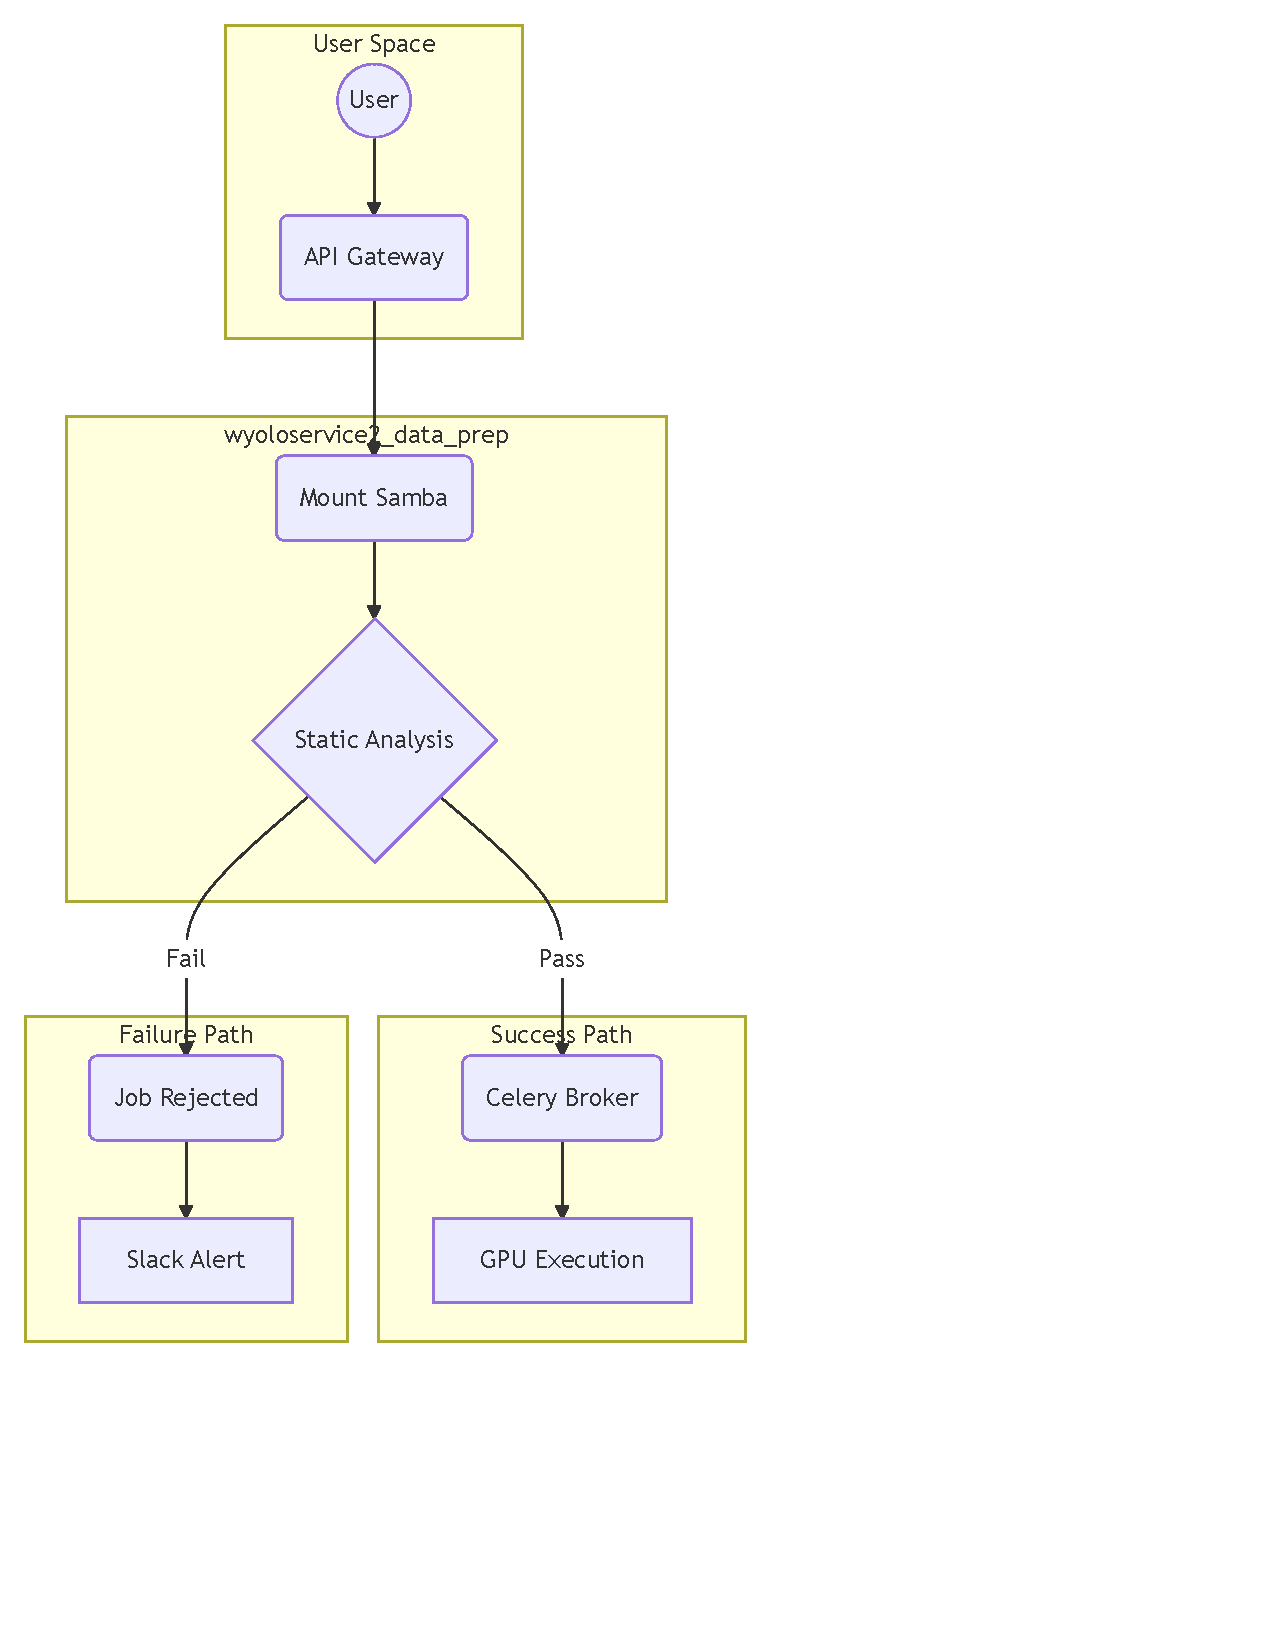
\includegraphics[width=\linewidth,height=0.3\textheight,keepaspectratio]{figures/gatekeeper.pdf}
\caption{Diagrama de flujo que muestra la lógica del Gatekeeper Shift-Left.}
\label{fig:gatekeeper}
\end{figure}

\section{Configuración Experimental y Detalles de Implementación}
Desplegamos el servicio \texttt{wyoloservice2\_data\_prep} en un nodo ligero de CPU de 4 núcleos, completamente separado del clúster de entrenamiento GPU de 3 nodos (RTX 4090s). Curamos un grupo de prueba de 100 conjuntos de datos YOLO. Corrompimos deliberadamente 30 de estos conjuntos de datos eliminando aleatoriamente archivos de etiquetas, inyectando etiquetas YAML malformadas, y agregando formatos de imagen no soportados (por ejemplo, \texttt{.tiff} sin encabezados).

Medimos las horas totales de GPU desperdiciadas por estos 30 conjuntos de datos corruptos en un canal heredado (Validación en Etapa Tardía) versus nuestro canal Shift-Left. También registramos el tiempo requerido para que un ingeniero humano diagnosticara la falla.

\begin{table}[htbp]
\centering
\caption{Grupo de Prueba de Conjuntos de Datos}
\label{tab:datasets}
\begin{tabular}{@{}lll@{}}
\toprule
Condición del Conjunto de Datos & Cantidad & Resultado Esperado \\ \midrule
Saludable & 70 & Reenviar a GPU \\
Etiquetas Faltantes & 15 & Rechazar vía Gatekeeper \\
YAML Malformado & 10 & Rechazar vía Gatekeeper \\
Imágenes Corruptas & 5 & Rechazar vía Gatekeeper \\ \bottomrule
\end{tabular}
\end{table}

\section{Resultados y Discusión}
La implementación del gatekeeper Shift-Left impactó profundamente la eficiencia del clúster y la velocidad de los desarrolladores.

\subsection{Estudio de Ablación: Desperdicio de GPU y Tiempo de Depuración}
Bajo la configuración heredada, los 30 conjuntos de datos corruptos evitaron cualquier control estructural y se cargaron directamente en las GPUs RTX 4090. Los cargadores de datos de PyTorch fallaron invariablemente durante la ejecución. Debido a que algunas corrupciones existían profundamente dentro del conjunto de datos, ciertos trabajos se ejecutaron durante más de 3 horas antes de llegar al archivo defectuoso y bloquearse. En total, estos 30 trabajos desperdiciaron 42.5 horas de cómputo de GPU. Además, diagnosticar las densas trazas de pila de PyTorch requirió un promedio de 2.4 horas de tiempo de ingeniería humana por incidente.

Con el gatekeeper \texttt{wyoloservice2\_data\_prep} activo, los 30 conjuntos de datos corruptos fueron interceptados inmediatamente. El análisis estático de CPU tomó un promedio de 4.2 segundos por conjunto de datos. Los trabajos fueron rechazados, y se desperdiciaron 0 horas de GPU. Las alertas automatizadas de Slack proporcionaron rutas exactas de archivos a la corrupción, reduciendo el tiempo de depuración humana a un promedio de 8 minutos.

\begin{table}[htbp]
\centering
\caption{Estudio de Ablación: Métricas de Desperdicio de Recursos}
\label{tab:ablation}
\begin{tabular}{@{}lll@{}}
\toprule
Métrica & Canal Heredado & Canal Shift-Left \\ \midrule
Horas de GPU Desperdiciadas & 42.5 & 0 \\
Tiempo Promedio de Depuración & 2.4 Horas & 8 Minutos \\
Sobrecarga Análisis CPU & 0 Seg & 4.2 Seg \\ \bottomrule
\end{tabular}
\end{table}

\begin{figure}[htbp]
\centering
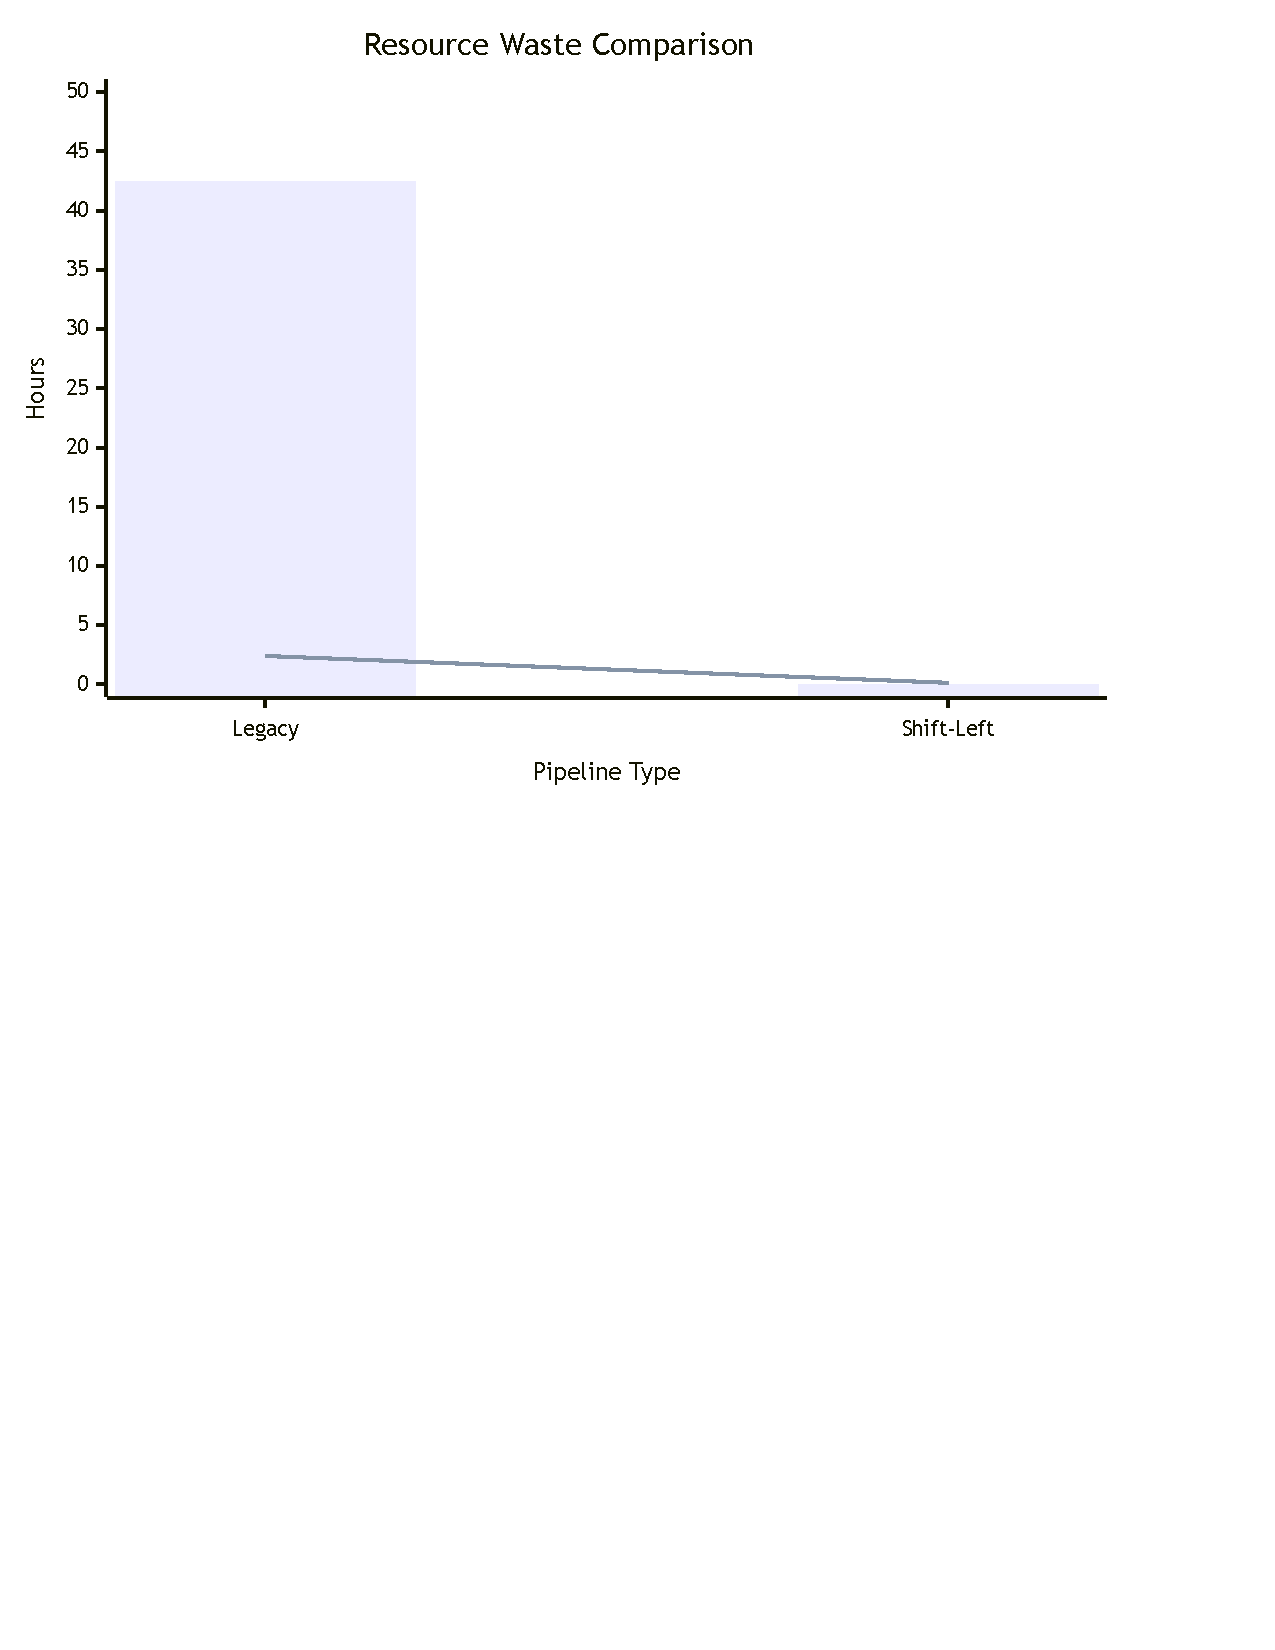
\includegraphics[width=\linewidth,height=0.3\textheight,keepaspectratio]{figures/waste_chart.pdf}
\caption{Gráfico de barras que compara las horas de GPU desperdiciadas y el tiempo promedio de depuración.}
\label{fig:waste_chart}
\end{figure}

\section{Declaración de Disponibilidad de Datos y Código}
Esta arquitectura opera bajo un Modelo de Licencia Dual (PolyForm No Comercial / AGPLv3). Para desplegar el proyecto y reproducir perfectamente estos experimentos declarados, se utiliza el repositorio \url{https://github.com/wisrovi/wyoloservice2_production}. Comandos de despliegue explícitos (por ejemplo, \texttt{docker-compose up -d}) están disponibles allí. Este repositorio sirve como un ejemplo concreto de cómo la investigación aplicada produce resultados excelentes y reproducibles para la comunidad.

\section{Impacto Más Amplio / Declaración de Ética}
Al imponer estrictas restricciones de calidad de datos antes de la ejecución, esta arquitectura reduce drásticamente el consumo de energía en los centros de datos de ML. Prevenir 42.5 horas de ejecución de GPU desperdiciada de 400W limita directamente las emisiones de carbono innecesarias. Adicionalmente, desplazar la validación a la izquierda obliga a los equipos de ingeniería de datos a mantener conjuntos de datos más limpios y responsables, alineándose con las prácticas éticas de curación de datos de IA.

\section{Conclusión y Trabajo Futuro}
Validar remotamente las estructuras de datos antes del entrenamiento es crítico para mantener la salud económica y operativa de un clúster de ML multi-inquilino. El servicio \texttt{wyoloservice2\_data\_prep} desplaza exitosamente esta carga a la izquierda, utilizando ciclos de CPU económicos para proteger recursos de GPU altamente valiosos. El trabajo futuro explorará la expansión del motor de análisis estático para detectar desequilibrios estadísticos y sesgos algorítmicos dentro del conjunto de datos antes de que se manifiesten en el modelo entrenado.

\section{Agradecimientos}
Extendemos nuestra gratitud a los contribuyentes del proyecto wisrovi-suit por proporcionar la infraestructura de orquestación fundacional que permitió esta integración.

\bibliographystyle{plain}
\bibliography{references}

\end{document}
